\documentclass[a4paper,11pt]{article}

\usepackage[utf8]{inputenc}
\usepackage[T1]{fontenc}
\usepackage{mathptmx}

\usepackage[a4paper,text={160mm,220mm},centering]{geometry}

\usepackage{hyperref}
\usepackage{listings}
\usepackage{graphicx}
\usepackage[table]{xcolor}

\lstset{basicstyle={\ttfamily}}

\usepackage{tikz}
\usepackage{pgf-pie}

\begin{document}


\unitlength=1mm
\begin{picture}(0,0)(0,10)
\put(-20,25){
\includegraphics[width=0.3\textwidth]{../images/Logo_Bpifrance.png}
  
\includegraphics[width=0.1\textwidth]{../images/Logo-France-2030-rouge-bleu.png}}
\end{picture}

\begin{center}\bfseries

  \Huge
  Projet Décysif --- Livrable 1.1

  \Large
  Constitution d’une base de fichiers d’entrée
représentatifs des difficultés rencontrées pour
générer des exploits.
\end{center}


Ce livrable est constituée d'une base de tests qui se trouve dans le dépot
\href{https://github.com/Decysif/benchmarks}{'benchmarks'} du projet Décysif.

Objectifs du livrable :

\begin{itemize}
\item Repérer les faiblesses du prouveur Alt-Ergo
\item Repérer les problèmes de traduction (ou repérer des problèmes au
  niveau de l'écriture des théories, par exemple le modèle mémoire de
  J3) pour tous les prouveurs cvc5, CVC4, Z3, Alt-Ergo.
\item Identifier des faiblesses lors de la reconstruction d'un
  contre-exemple par Why3 depuis les modeles des solveurs
  SMT~\cite{dailler18jlamp}
\item Identifier les faiblesses des procédures de vérification et
  catégorisation des contre-exemples~\cite{becker21rr,becker21fide}
\end{itemize}

% Une section par répertoire d'exemples avec une description du contenu
% et de la méthodologie des statisques adoptée. Et le résultat de ces statisques
% au démarrage du projet.

% Mettre les statistiques qu'on a quand elles existent.

\section{Contre-Exemples générés sur du code  WhyML}

Le jeu de tests sur les contre-exemples en Why3 s'appuie sur
l'installation locale de Why3 qui est déjà décrite dans le livrable
1.2. Donc si ce n'est pas déjà fait, il faut installer et configurer Why3 en allant dans le répertoire \url{why3_exemple} et exécuter
\begin{lstlisting}
> ./import_suite.sh
\end{lstlisting}

\subsection{Suite de tests issues de Why3}

La suite de tests pour les contre-exemples se trouvent dans le
répertoire \url{why3_ce}. Il faut initialiser la suite de tests en
allant dans ce répertoire et exécuter
\begin{lstlisting}
> ./import_suite.sh
\end{lstlisting}
(il s'agit d'un autre script que le précédent)

Les tests peuvent ensuite être exécutés par la commande
\begin{lstlisting}
> ./run_bench.sh
\end{lstlisting}
Les resultats des tests sont stockés dans le sous-répertoire
\url{tests}. Des statistiques peuvent être calculées pour synthétiser
les résultats de ce tests, avec le script
\begin{lstlisting}
> ./ce-stats.py
\end{lstlisting}
qui génère des fichiers de statistiques au format CSV.

Une exécution de ces tests a été effectuée
le 22 avril 2024, avec les prouveurs Alt-Ergo 2.5.2, CVC4 1.8, CVC5
1.0.5 et Z3 4.8.10. les résultats globaux sont donnés par la table ci-dessous.
  \begin{center}
  \rowcolors{2}{gray!25}{white}
  \begin{tabular}{|l|r|r|}
  \rowcolor{gray!50} Verdict
  & \multicolumn{1}{p{0.13\textwidth}|}{nombre d'occurrences}
  & \multicolumn{1}{p{0.13\textwidth}|}{pourcentage}
  \\
Non-Conformity         & 721 & 61,36 \% \\
Specification Weakness & 93 & 7,91 \% \\
    NC or SW  	       & 6 & 0,51 \% \\
Bad Counterexample & 195 & 16,60 \% \\
    Validation Incompleteness & 160 & 13,62 \%
  \end{tabular}
\end{center}
Ces statistiques sont également visualisées par le diagramme
  suivant.
  \begin{center}
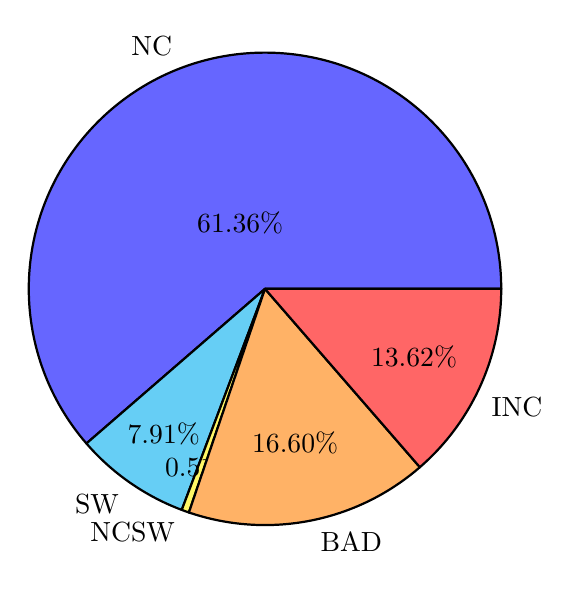
\begin{tikzpicture}
    \pie{61.36/NC, 7.91/SW, 0.51/NCSW, 16.60/BAD, 13.62/INC}
\end{tikzpicture}
\end{center}
La première ligne (Non-Conformity) désigne les cas où une erreur de
code à été effectivement identifiée, plus précisément un cas où le
code n'est pas conforme à la spécification, et où un contre-exemple
explicite est produit pour générer l'exploit correspondant. La seconde
ligne (Specification Weakness) concerne les cas où un contre-exemple
est généré mais qui ne révèle pas un exploit mais une insuffisance
dans les spécifications (manque d'invariant de boucle où
sous-spécification d'une fonction auxiliaire) qui emphe de faire une
preuve. Ces deux cas sont des cas favorables, et on va chercher à
augmenter leurs fréquences. Le cas ``NC or SW'' est un cas où l'on
n'arrive pas à décider si le contre-exemple est un exploit où bien si
c'est une faiblesse de spécification. C'est aussi une situation
favorable mais si plus imprécise. le cas Bad Counterexample est
défavorable: le contre-exemple proposé par le solveur n'est en fait
pas un bon contre-exemple, et ce fait a été détecté comme tel par la
procédure de validation. On souhaite diminuer le pourcentage de ces
cas, et la seule façon que l'on a pour réduire ce pourcentage est de
modifier les tâches de preuve que l'on soumet au solveur, afin que
celui-ci soit plus performant. Le dernier cas Validation
Incompleteness est aussi défavorable et on va chercher à le
diminuer. Pour cela, il faut jourer sur la méthodologie actuelle pour
valider les contre-exemples, telle qu'implémentée dans Why3.  Le taux
de cas favorables est de l'ordre de 70 \%, et l'augmentation de ce
taux est donc un objectif général.

Pour le dernier cas ``Validation Incompleteness'', on peut donner des
statistiques plus détaillées. Voici ces statistiques pour la partie de
validation dite ``à petits pas''
  \begin{center}
  \rowcolors{2}{gray!25}{white}
  \begin{tabular}{|l|r|r|}
  \rowcolor{gray!50} Réponse
  & \multicolumn{1}{p{0.65\textwidth}|}{explication}
  & \multicolumn{1}{p{0.13\textwidth}|}{nombre d'occurrences}
    \\
INCOMPLETE & cannot decide	& 127 \\
INCOMPLETE & missing return value & 11 \\
INCOMPLETE & uncaught exception	& 8 \\
INCOMPLETE & (terminated because mlmpfr wrapper is not implemented) & 6 \\
INCOMPLETE & many args for exec	& 2 \\
INCOMPLETE & (terminated because index is out of bounds) & 1 \\
INCOMPLETE & (terminated because missing value for global `get`) & 1 \\
\end{tabular}
\end{center}
Les deux premières lignes correspondent à des améliorations à apporter
à la méthodologie. Les autres lignes correspondent a priori tout
simplement à des bugs qu'il faut corriger.

Les statistiques pour la
partie de validation dite ``à pas de géant'' sont les suivantes.
\begin{center}
  \rowcolors{2}{gray!25}{white}
  \begin{tabular}{|l|r|r|}
  \rowcolor{gray!50} Réponse
  & \multicolumn{1}{p{0.65\textwidth}|}{explication}
  & \multicolumn{1}{p{0.13\textwidth}|}{nombre d'occurrences}
    \\
INCOMPLETE & cannot decide	& 129 \\
INCOMPLETE & missing return value  &	15 \\
INCOMPLETE & uncaught exception	& 8 \\
INCOMPLETE &  (terminated because mlmpfr wrapper is not implemented) &	6 \\
INCOMPLETE & (terminated because index is out of bounds) &	1 \\
    INCOMPLETE & (terminated because missing value for global `get`) &	1 \\
  \end{tabular}
\end{center}
Les conclusions sont les mêmes que pour la partie petits pas: deux
pistes d'amélioration, et des bugs à corriger.


\subsection{Suite de tests construits à la main}

Une autre base de tests est construite manuellement dans l'objectif d'améliorer
la façon de présenter un contre-exemple. Cette restitution est importante pour
un utilisateur de Why3 mais aussi pour les différents front-end pour le C ou
pour Ada. Ce jeu de tests est donné dans le sous-répertoire \url{tests_for_log}
du répertoire \url{why3_ce}. Pour ces tests on ne mesure pas leur succès par des
statistiques mais par une proximité avec un résultat attendu. Les résultats
attendus pour ces tests seront décrits dans un livrable annexe à celui-ci d'ici
la fin 2024 au plus tard.  \footnote{Les sources de cette annexe sont
  actuellement dans le sous-repertoire \url{counterexamples} du dépôt
  \url{livrables}}

\section{Contre-Exemples issus de J3}

TODO [Guillaume]

Méthodologie pour extraire des statistique à décrire

\section{Contre-Exemples issus de SPARK}

TODO [Yannick]


\section{Travail futur}

Quelles autres statistiques peut-on vouloir?

Creer une infrastrcture de contre-exemples pour Creusot

\clearpage

\bibliographystyle{plainurl}
\bibliography{generated,main}
%\bibliography{abbrevs,demons,demons2,demons3,team,crossrefs}

\end{document}


% Local Variables:
% mode: latex
% mode: flyspell
% TeX-master: t
% TeX-PDF-mode: t
% ispell-local-dictionary: "francais"
% fill-column: 80
% End:
